\documentclass[a4paper, 12pt, addpoints]{exam}

\usepackage{fontspec}   %加這個就可以設定字體
\usepackage{xeCJK}       %讓中英文字體分開設置
\usepackage{float}
\usepackage{graphicx}
\usepackage{caption}
\usepackage{hyperref}
\usepackage{amsmath}
\usepackage{multirow}

\usepackage[dvipsnames]{xcolor}
\usepackage{graphicx}
\usepackage{tabularx}
\usepackage{bookmark}
\usepackage{adjustbox}

\usepackage[utf8]{inputenc}
\usepackage{graphics}
\usepackage{color}
\usepackage{amssymb}
\usepackage{amsmath}
\usepackage{enumitem}
\usepackage{xcolor}
\usepackage{graphicx}
\usepackage{multicol}
\usepackage{color}
\usepackage{tikz}
\usepackage[randomizechoices, overload]{exam-randomizechoices} % to make random order choices

\usetikzlibrary{calc}
\newcommand*{\TickSize}{2pt}%



\usepackage[
    right=1.5cm,
    left=1.5cm,
    top=2cm,
    bottom=2cm
]{geometry} 



\CorrectChoiceEmphasis{\color{red}}

\pointpoints{分}{分}


\setCJKmainfont{Noto Sans CJK TC}
\setmainfont{Times New Roman}
% \setmonofont{CascadiaCode.ttf}
\setmonofont{Consolas}
\XeTeXlinebreaklocale "zh"             %這兩行一定要加,中文才能自動換行
\XeTeXlinebreakskip = 0pt plus 1pt     %這兩行一定要加,中文才能自動換行

% \addfontfeatures{FakeBold=1.5}

\setlength{\parskip}{0.5em} % 段落間0.5字元

\renewcommand{\baselinestretch}{1.5}
\setlength\linefillheight{2em}

\renewcommand\choicelabel{(\Alph{choice})}

\pagestyle{headandfoot}
\runningfooter{}
{\thepage\ of \numpages}
{}

\begin{document}


\begin{coverpages}

    %---uncomment to add a custom header (replace {header-cufm.png})---- %
    %\begin{figure}[t]
    %\includegraphics[width=1\textwidth,height=1.2\textheight,keepaspectratio]{%header-cufm.png}
    %\end{figure}

    \begin{center}
        {\huge 110 武陵資訊讀書會 \\ 運算思維及邏輯能力測驗}
    \end{center}

    \begin{center}
        \fbox{\fbox{\parbox{6in}{
                    \begin{itemize}[leftmargin=*]
                        \item 考試時間:x分鐘
                        \item 試題分四部分,第一部分為選擇題,\underline{\textbf{共7題,28分}}、第二部分為填充題,\underline{\textbf{共9題,36分}}、第三部分為邏輯論述題,\underline{\textbf{共3題,16分}}、第四部分為題組題\underline{\textbf{共2題,20分}}。
                    \end{itemize} }}}
        \vspace{\stretch{1}}

        \makebox[0.45\textwidth]{班級:\enspace\hrulefill}

        \makebox[0.45\textwidth]{姓名:\enspace\hrulefill}
    \end{center}
    \vspace{0.15in}
    \runningheadrule \extraheadheight{0.14in}


    \vspace{0.15in}

    \vspace{0.1in}

    %-comment out the next line to display point value for each question -%
    \nopointsinmargin
    \setlength\linefillthickness{0.1pt}
    \setlength\answerlinelength{0.1in}
\end{coverpages}

\noindent \textbf{\large 第一部分:選擇題(佔 28 分)}

\noindent \fbox{\parbox{\dimexpr\linewidth-2\fboxsep-2\fboxrule\relax}{說明:每題答對得 4 分,\textbf{答錯倒扣 2 分},未作答得 0 分。}}%

\vspace{0.1in}
\begin{questions}
    \question[4]
    奇異果高中宿舍有5層樓,每層有8間房。清掃機器人會遵循以下的指令:

    \begin{itemize}
        \item 指令C:搜尋這一層樓任何一間尚未清潔過的房間,並把它們清掃乾淨。
        \item 指令U:往上一層樓。
        \item 指令D:往下一層樓。
    \end{itemize}



    整數 n (指令):表示重複做括弧內的指令 n 次,括弧內可以有一個以上的指令。

    舉例來說,如果你想讓機器人在同一樓層清掃兩個未清潔過的房間,請輸入2(C)。如果你希望機器人清掃完這兩個房間後,接下來往下一層樓,就要輸入2(C) D。

    為了確保機器人會清掃完飯店的所有房間,機器人必須從客房第一層樓開始,結束也回到第一層樓,未清掃完同一樓層所有房間前不能到其他樓層。

    請注意機器人在遇到無法執行指令的情況,就會自動停止不再執行:包括這一層樓的房間都已清理過卻收到指令C,在第五層樓收到指令U,或在第一層樓收到指令D。

    請問下列哪個選項中的指令能正確地讓機器人完成這項任務?

    \begin{choices}
        \choice 4(8(C) U) 8(C) 4(D)
        \choice 4(8(C) U) 8(C D)
        \choice 5(8(C) U) 4(D)
        \choice 5(C) U 4(D)
    \end{choices}

    \question[4] 熊熊和閎閎在4乘4的大板子上玩L遊戲,熊熊和閎閎輪流將L型的木片放在大板子上,遊戲規則如下:

    \begin{itemize}
        \item 熊熊所放的木片方向如下所示。
        \item 閎閎所放的木片方向如下所示。
        \item 任何木片都不能超出大板子外。
        \item 木片和木片之間不能重疊。
    \end{itemize}

    \begin{figure}[H]
        \centerline{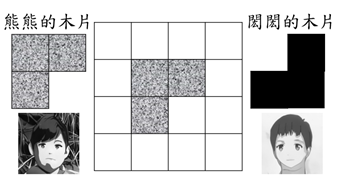
\includegraphics{fig/p2.png}}
    \end{figure}

    木片被放到大板子上後不能再被移動。假設熊熊已在大板子上放第一片木片(如上圖所示),閎閎將放第二片,依此類推,最後無法再放木片的人便是輸家。

    下列敘述何者正確?

    \begin{choices}
        \choice 熊熊一定會獲勝
        \choice 閎閎一定會獲勝
        \choice 兩人都可能獲勝,但熊熊獲勝的機率較高
        \choice 兩人都可能獲勝,但閎閎獲勝的機率較高
        \choice 熊熊和閎閎的獲勝機率相同
    \end{choices}

    \question[4] 美國聖地亞戈農資集團的第⼀代創辦人美美因為調配出能吸收兩米下氮磷鉀的肥料──金坷垃──因此振興了非洲農業。為了避免太多人知道金坷垃的秘傳配方,美美規定,交接給下一代時,一個人最多只能告訴兩位最值得信任的幹部金坷垃的秘傳配方。請問,公司傳到第 8 代時, 最多有幾個人知道金坷垃的秘傳配方?(第一代幹部中只有美美知道金坷垃的配方)

    \begin{choices}
        \choice 255
        \choice 256
        \choice 511
        \choice 512
    \end{choices}

    \question[4] 從前從前,頂樓加蓋的違章建築就已經是中華民國美學中不可或缺的一部分了。萬萬沒想到,市長居然要開拆了!但拆除違章建築也不是那麼容易,必須逐次進行,並符合以下規則:

    \begin{itemize}
        \item 如果違建的旁邊都沒有違建,那就可以直接拆除。

              \adjustbox{valign=t}{
\includegraphics{fig/p41.png}}

        \item 如果違建的其中一邊沒有違建,那也可以直接拆除。

              \adjustbox{valign=t}{
\includegraphics{fig/p42.png}}

        \item 一次可以拆除多棟違建。

              \adjustbox{valign=t}{
\includegraphics{fig/p43.png}}

        \item 如果違建的兩邊都有違建,就暫時不能拆除,需要等其中一邊被拆掉後,下一次才能拆它。

              \adjustbox{valign=t}{
\includegraphics{fig/p44.png}}
    \end{itemize}
    由於柯市⻑急著做出政績,想要快速拆光⼀整條路上的違建。請問以下哪⼀條路拆光所需要的次數最少?
    \begin{choices}
        \choice \adjustbox{valign=t}{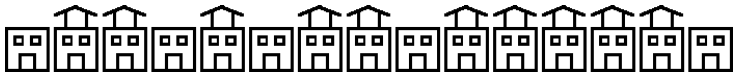
\includegraphics[width=0.5\textwidth]{fig/p4a.png}}
        \choice \adjustbox{valign=t}{
\includegraphics[width=0.5\textwidth]{fig/p4b.png}}
        \choice \adjustbox{valign=t}{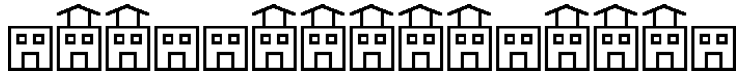
\includegraphics[width=0.5\textwidth]{fig/p4c.png}}
        \choice \adjustbox{valign=t}{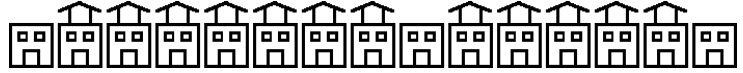
\includegraphics[width=0.5\textwidth]{fig/p4d.png}}

    \end{choices}

    \question[4] 熊熊有兩個水杯,分別為$x$公升與$y$公升,今天可以對水杯做下列幾種操作:
    \begin{itemize}
        \item 裝滿任一水杯裡的水
        \item 倒掉任一水杯裡所有的水
        \item 把⼀個⽔杯裡的⽔,倒進另⼀個⽔杯中,直到沒有⽔,或是另⼀個⽔杯滿了為⽌
    \end{itemize}

    如果熊熊想要得到恰好 $z$ 公升的⽔,那下列哪種可能是有辦法完成的?

    \begin{choices}
        \choice $x=4, y=2, z=3$
        \choice $x=21, y=3, z=10$
        \choice $x=7, y=8, z= 10$
        \choice $x=2, y=12, z=3$
    \end{choices}

    \question[4]
    Howard 喜歡使⽤社群軟體,⽽且他喜歡經營多個帳號,可以讓他在網路上有多個⾝份。最近 Howard 發現了⼀個名叫 infor 的社群軟體,註冊 infor 時需要輸⼊使⽤者暱稱,規定只能由⼩
    寫英⽂字⺟ (a$\sim$z) 組成,⽽且必須是還沒被使⽤過的暱稱。

    當 Howard 在煩惱有什麼暱稱可以使⽤時,他想到了⼀個辦法:

    他把每個英⽂字⺟編號,$a = 1, b = 2, c = 3, \cdots, z = 26$,接著他把⾃⼰的名字依照編號轉換成    數字:$a(1)r(18)v(22)i(9)n(14) \ \rightarrow \ 11822914$,最後把這⼀串數字依照編號轉換回英⽂字⺟,作為
    暱稱。

    例如⼀種可能的⽅式是 $1,1,8,2,2,9,1,4 \rightarrow aahbbiad$。請問由 Howard 的想法,他可以產⽣多少不同暱稱?

    \begin{choices}
        \choice 6
        \choice 8
        \choice 12
        \choice 20
    \end{choices}

    \question[4]
    Piepie 是⼀位職業撲克牌玩家,常常出沒於世界各個⾓落,把⼀些沒良⼼的有錢⼈、政客的錢賺⾛。就算是如此神奇的⼈,也是會有懶的時候,他最討厭做的事就是抬起⼿去整理牌了,但是⼜得要好好的把牌排好,不然失誤反⽽錢被騙⾛就糟了,所以他練就了⼀招——偷天換⽇。「偷天換⽇」會在 Piepie 眨⼀下眼的時候,無形之中將兩張相鄰的牌互換位置。

    以下是他的手牌:
    \begin{figure}[H]
        \centerline{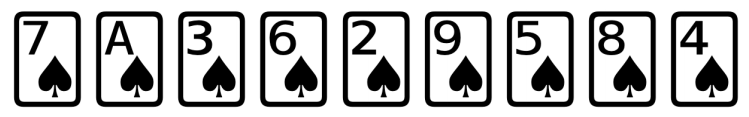
\includegraphics[width=0.75\textwidth]{fig/card.png}}
    \end{figure}


    請問他最少需要使⽤多少次「偷天換⽇」才能將上⾯的牌照順序排好(由 A 到 9 從左⾄右排序)?


    \begin{choices}
        \choice 13
        \choice 15
        \choice 17
        \choice 19
    \end{choices}
\end{questions}

\newpage
\noindent \textbf{\large 第二部分:填充題(佔 36 分)}

\noindent \fbox{\parbox{\dimexpr\linewidth-2\fboxsep-2\fboxrule\relax}{說明:每題完全答對得 4 分,部分答對、答錯或未作答得 0 分。}}%

\vspace{0.1in}
\begin{questions}
    \question[4]
    奇異果高中的運動會中有一個趣味競賽項目,在操場的圓形跑道上,每隔一段距離會放一個寶物,每個寶物都標有代表分數,有些是正分也有些是負分。比賽規則如下:選手可以選擇從操場任一處進入圓形跑道,進入跑道若要開始撿拾寶物,就要蹲下用蹲走的方式,蹲走所遇到的寶物都要撿拾,一旦站起來後就不能再撿拾寶物,得分為所有撿拾寶物的分數加總。現在將標有以下分數的寶物依序擺放在圓形跑道上,請問此項趣味競賽能夠得到的最高總分是多少?

    \begin{figure}[H]
        \centerline{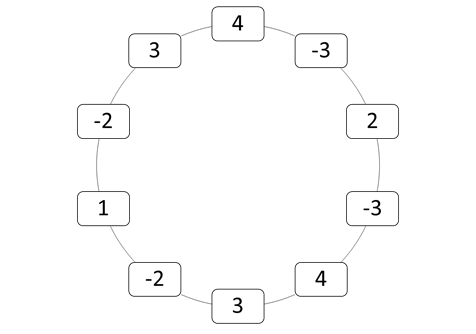
\includegraphics{fig/sports.png}}
    \end{figure}

    \question[4]
    閎閎是個小迷糊,總是忘記帶東西。每天他上學(或放學)時若下雨,他就會記得帶一支傘;但若放學時沒下雨,他就會忘記把傘帶回家;如果上學時沒下雨,他也不會帶傘。若開學前的返校日可以先準備一些傘分別放在學校和家裡,請問他最少總共需要準備幾支傘,才不會在開學頭三天上學或放學的時候,遇到下雨但手邊沒傘?


    \question[4]
    有一隻在數線上左右跳動的青蛙,每次向左跳動跟向右跳動的間隔數不一,定義如下方的程式所示。程式執行時會輸出每次青蛙跳動後的位置。若青蛙從位置1開始,重複以下的過程,2$\sim$10會有一個位置沒有被輸出,請問是哪個位置?

    \begin{figure}[H]
        \centerline{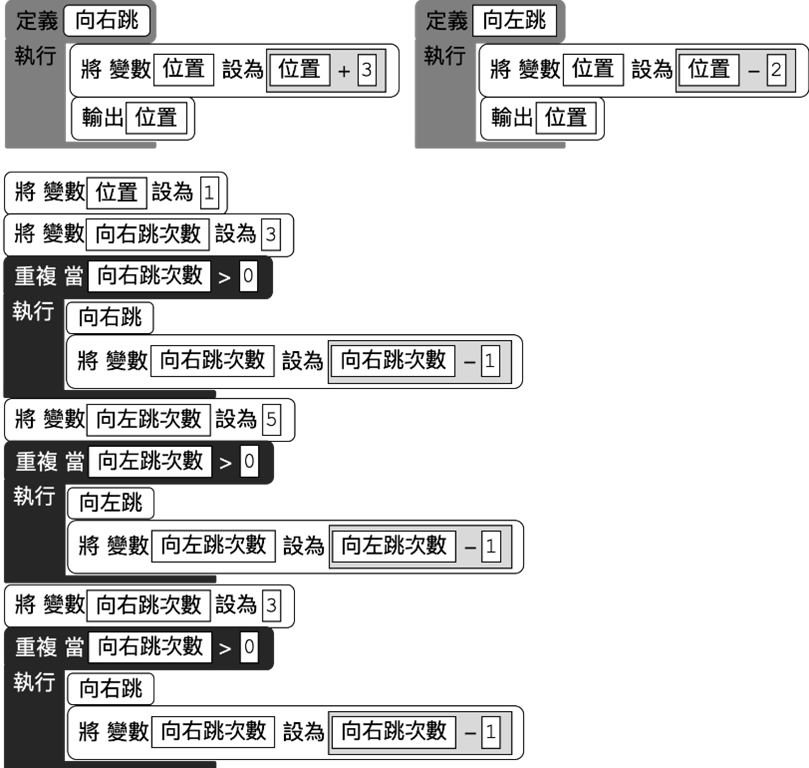
\includegraphics{fig/frog.png}}
    \end{figure}

    \question[4]
    西洋棋中的皇后可以縱向、橫向、斜向任意移動。學習遞迴時會碰到八皇后問題,就是在一個8×8的方格棋盤上放置八個皇后棋,使得任一個皇后棋不被其他的皇后吃掉,也就是棋盤中的每一個縱向、橫向、斜向都只能放置一個皇后棋。舉例來說,左下圖的八個皇后就滿足上述問題的要求。

    \begin{figure}[H]
        \centerline{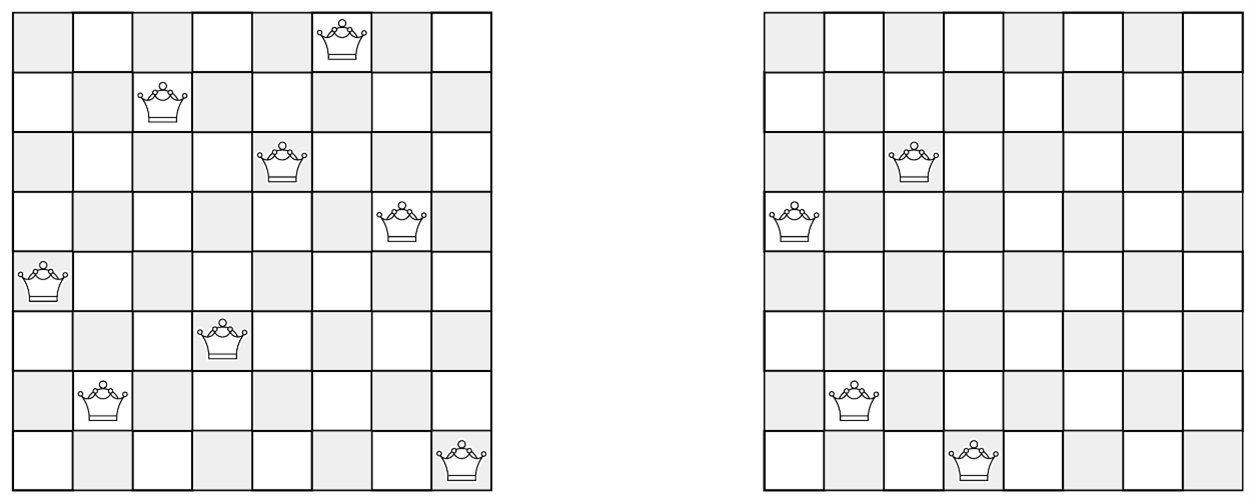
\includegraphics{fig/chess.png}}
    \end{figure}
    右上圖中的八個皇后棋已經放置四個,請問其餘的四個皇后棋有多少種不同的放置方式能滿足八皇后問題的要求呢?


    \question[4]
    花栗鼠們囤積了許多栗子。花栗鼠國有個習俗,一定要按照以下的方法將栗子分堆:

    \begin{itemize}
        \item 一堆任意數目的栗子,要平分成數量一樣,或只相差1顆的兩堆;
        \item 若一堆栗子數量多於2顆,就要繼續分堆;
        \item 如果發現有兩堆栗子各只有1顆,則這兩堆會被合併成一堆。
    \end{itemize}

    例如下圖所示:當栗子總數為10顆時,則分堆過程如左圖示,共會進行5次分堆及一次合併;當栗子總數為9顆時,則分堆過程如右圖示,共會進行4次分堆。
    \begin{figure}[H]
        \centerline{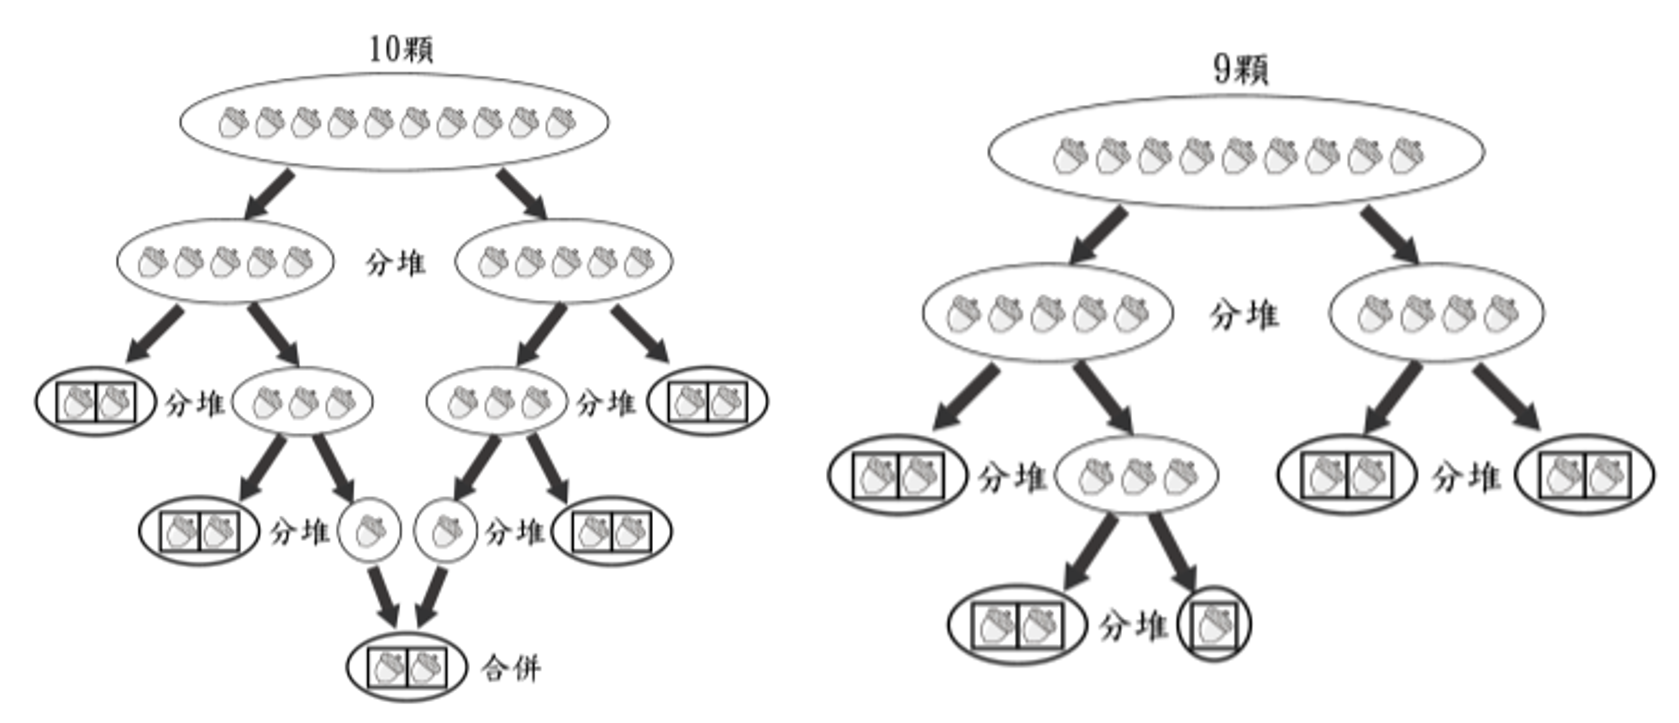
\includegraphics[width=\textwidth]{fig/sq.png}}
    \end{figure}

    若栗子總數量為125顆,則共會進行A次分堆及B次合併?


    \question[4]
    走廊上的電梯旁一列整齊排放的奇異果籃,每籃旁邊標示著該籃的重量(公斤),如下表。

    \begin{table}[H]
        \centering
        \resizebox{0.75\textwidth}{!}{%
            \begin{tabular}{|c|c|c|c|c|c|c|c|c|c|c|c|c|}
                \hline
                15 & 30 & 25 & 10 & 30 & 45 & 23 & 50 & 55 & 34 & 20 & 40 & 電梯 \\ \hline
            \end{tabular}%
        }
    \end{table}
    熊熊依下列規則將奇異果籃以電梯運送到三樓辦公室:

    \begin{itemize}
        \item 電梯每趟運送都需裝載80至100公斤的奇異果籃,最後一趟可裝載低於80公斤。
        \item 裝載奇異果籃時,須從最靠近電梯的籃子依序裝載。
        \item 若某籃導致電梯超重,則把該籃放到該列奇異果籃的最後面。
    \end{itemize}

    請問電梯最少需運送幾趟才能將所有的奇異果籃送到辦公室?

    \question[4]
    武陵高中美池下有個防空洞,共有四個洞穴(A、B、C、F),其中F洞穴是避難室。在部分洞穴間設有坑道。某天,共匪打來了,有10個人在A洞穴,而他們想盡快到F洞穴避難。通過一條坑道到另一個洞穴需要1分鐘,但每條坑道同一時間只能有一個人通行。

    洞穴之間有特定數量的坑道連接,如下圖所示:
    \begin{figure}[H]
        \centerline{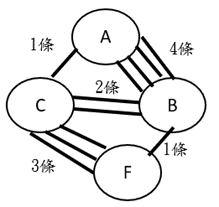
\includegraphics{fig/cave.png}}
    \end{figure}


    每個洞穴都沒有容量限制,也就是每個洞穴可容納無限個人。
    要讓所有人都到達避難室,最短需要幾分鐘?

    \question[4]
    Winecraft遊戲中,有著豐富的葡萄錠,酒商會在葡萄園採收,並請神職人員(cleric)將葡萄錠融合成更大的葡萄錠,方便外銷。

    神職人員每次只能融合兩顆葡萄錠,而且會依據融合後葡萄錠的重量收取費用,收費標準是1公克1顆綠寶石。假設手上有5顆葡萄錠重量分別為5公克、7公克、6公克、3公克和2公克。如果依照以下步驟融合葡萄錠:
    \begin{enumerate}
        \item 將5公克和7公克的葡萄錠融合成12公克的葡萄錠,需花費12顆綠寶石。
        \item 將6公克和3公克的葡萄錠融合成9公克的葡萄錠,需花費9顆綠寶石。
        \item 將12公克(步驟1的結果)和9公克(步驟2的結果)的葡萄錠融合成21公克的葡萄錠,需花費21顆綠寶石。
        \item 將21公克(步驟3的結果)和2公克的葡萄錠融合成23公克的葡萄錠,需花費23顆綠寶石。
    \end{enumerate}
    \begin{figure}[H]
        \centerline{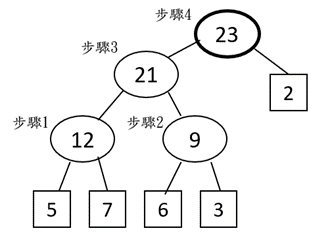
\includegraphics{fig/wine.png}}
    \end{figure}


    總共花費$12+9+21+23=65$顆綠寶石。但同樣的這5顆葡萄錠如果按照另一種順序,($5+7=12$公克,$3+2=5$公克,$12+5=17$公克,$17+6=23$公克)就只要$12+5+17+23=57$顆綠寶石。

    假設手上目前有8顆葡萄錠,重量分別是7公克、1公克、3公克、2公克、6公克、2公克、5公克、4公克。請問要將這8顆葡萄錠融合成1顆葡萄錠,所需要的最少花費是多少?

\end{questions}


\newpage
\noindent \textbf{\large 第三部分:邏輯論述題(佔16分)}

\noindent \fbox{\parbox{\dimexpr\linewidth-2\fboxsep-2\fboxrule\relax}{說明:請寫出完整過程,否則不予給分。若字跡過醜或書寫順序雜亂以致無法辨識,請自行負責。}}%


\vspace{0.1in}
\begin{questions}
    \question[6]
    九顆彈珠中有一顆比其他八顆重一點,請問如何用天平秤最小次數就可以把比較重的彈珠找出來?
    \question[3]
    熊熊肚子餓了想煎牛排吃,他有一個鍋子,最多可以同時煎兩塊牛排。煎熟一面牛排需$k$分鐘,兩面煎熟需$2k$分鐘。現在有$n$塊牛排,$n$為任一大於2的正整數,請問如何在最短時間內煎完$n$塊兩面都熟的牛排?(3分)
    \question[7]
    總共有5個人,其中兩個人一定不會說謊,三個人一定會說謊,請依照下面敘述,判斷誰在說謊,並寫出完整推理過程。

    甲:乙說謊

    乙:丙說謊

    丙:戊說謊

    丁:甲乙說謊

    戊:乙丙說實話


\end{questions}

\newpage
\noindent \textbf{\large 第四部分:題組題(佔 20 分)}
\vspace{0.15in}
\hrule
\vspace{0.1in}
\begin{questions}
    \question[12] COSINE-19肆虐,孜獨國政府為了防止疫情在國內散布,加強邊境管制。所有凡是從苗栗回國的人,都必須接受14天的自主隔離。此外,若曾經與確診患者接觸者,也必須自主隔離14天。

    孜獨國流行疫情指揮中心提供了入境者的接觸資料,而由於系統出錯,只能顯示前序(Prefix)遍歷和中序(Infix)遍歷後的資料。前序遍歷拜訪順序為根節點(A)$\rightarrow$左子節點(B)$\rightarrow$右子節點(C),拜訪到A的左子節點B時又可將B視為根節點,以上述方法繼續拜訪;中序遍歷拜訪順序為左子節點(B)$\rightarrow$根節點(A)$\rightarrow$右子節點(C)。例如若要調閱入境者A的資料會顯示Prefix:ABDCEF  Infix:DBAECF,即依照前序或中序遍歷拜訪順序輸出。

    \begin{figure}[H]
        \centerline{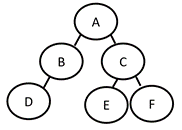
\includegraphics[width=0.5\textwidth]{fig/covid.png}}
    \end{figure}


    接觸的定義是與該人相連的人,例如與C接觸的有A、E、F三人,而與D接觸的只有B。

    已知在這份接觸資料中,發現任一人的上一接觸者最多只有1人,且下一接觸者最多2人(例如C的上一接觸者為A,C的下一接觸者為E和F)

    請問:熊熊於某天從苗栗回國時,被疾管署要求自主隔離14天,而調閱資料後,得知部分的接觸資料為Prefix:ABGDKHCGFIJMG  Infix:KDGHBAGCIFMJG。

    \begin{parts}
        \part[3] 代表熊熊的字母是?
        \part[9] 若調閱後過了14天,發現熊熊沒有任何症狀而解除隔離,反而G被確診得到COSINE-19,有哪些字母的人必須被自主隔離?(答案請依A-Z寫出)(Hint:觀察範例,試著找出規則) (全對得9分,錯$k$個得$9–2^k$分,錯4個以上得0分)
    \end{parts}

    \question[8] 閱讀下列資料後,回答問題:

    對於一個帶有整數參數 $n$ 的命題 $P(n)$,若我們希望證明對於所有的 $n \geq c$,$P(n)$皆成立 (為真),則只要證明以下兩點即可:
    \begin{enumerate}
        \item $P(c)$為真
        \item 對於所有$k \geq c$,若$P(k)$為真,則$P(k+1)$也為真
    \end{enumerate}

    為什麼這樣就證明完了呢?我們可以想一下,要怎麼證明「對於所有 $n \geq c$,$P(n)$都成立」這種命題?當然一開始可以先代入前幾項,也就是 $P(c), P(c + 1), P(c + 2)$,一個一個慢慢嘗試,發現真的全部都成立,但是這樣並不構成一個證明,畢竟誰知道他不會在 $P(c + 10000)$ 的時候就不成立了呢?當然,如果把所有大於等於 $c$ 的整數都代入過就可以證明 (窮舉法),但是這樣的數有無窮多個,這個方法當然不可行。

    數學歸納法的精神就像推骨牌一樣。想像每個整數都是一張骨牌,而現在你想證明所有的骨牌都會倒下,但是從上面的描述可以知道,一張一張證明是永遠都證明不完的,因此我們換個方法:
    \begin{enumerate}
        \item 證明第一張骨牌會倒下
        \item 證明如果一張骨牌倒下了,這張骨牌之後的下一張骨牌也一定會倒下
    \end{enumerate}
   
    這樣是不是就證明了所有骨牌都會倒下了呢?因為第一張骨牌倒了,第二張也會倒;因為第二張倒了,第三張也會倒…如此一來,所有的骨牌一定都會倒下了。特別一提的是,一定要兩個條件都滿足,證明才會成立。如果只證明了第一點,則無法保證後面的骨牌也會倒下;如果只證明了第二點,則第一張骨牌可能沒倒,這樣後面就沒戲唱了。

    大家可以發現,數學歸納法與大家熟悉的遞迴關係,本質其實是一樣的,數學歸納法中的初始條件可以想像成遞迴關係的終止條件,逐步遞推也就是遞迴中問題的拆解。換句話說,其實遞迴關係的正確性就是基於數學歸納法所證明的!數學歸納法在遞迴關係的證明上是非常好用的工具,希望大家好好體會一下。
    \begin{parts}
        \part[4] 證明對於至少為4的正整數$n$,滿足$n!>2^n$
        \part[4] 請證明:$\displaystyle \sum_{i=0}^{n} 2^i=2^{n+1}-1 (n \geq 0)$
    \end{parts}
\end{questions}

\begin{center}
    \textbf{\Large 試題結束,請記得將答案填寫於答案卷上。}
\end{center}

\newpage

\begin{center}
    \huge \textbf{答案卷}
\end{center}

\noindent \large \textbf{選擇題}
\begin{table}[H]
    \resizebox{0.45\textwidth}{!}{%
    \begin{tabular}{|l|l|l|l|l|l|l|}
    \hline
    1 & 2 & 3 & 4 & 5 & 6 & 7 \\ \hline
      &   &   &   &   &   &   \\ \hline
    \end{tabular}%
    }
\end{table}

\noindent \large \textbf{填充題}
\begin{multicols}{2}
\begin{enumerate}[leftmargin=*]
    \item \makebox[0.3\textwidth]{\enspace\hrulefill}
    \item \makebox[0.3\textwidth]{\enspace\hrulefill}
    \item \makebox[0.3\textwidth]{\enspace\hrulefill}
    \item \makebox[0.3\textwidth]{\enspace\hrulefill}
    \item \makebox[0.3\textwidth]{\enspace\hrulefill}
    \item \makebox[0.3\textwidth]{\enspace\hrulefill}
    \item \makebox[0.3\textwidth]{\enspace\hrulefill}
    \item \makebox[0.3\textwidth]{\enspace\hrulefill}
\end{enumerate}
\end{multicols}

\noindent \large \textbf{邏輯論述題}

\begin{enumerate}[leftmargin=*]
    \item \hspace{1em}  
    \fillwithlines{8em}
    \item \hspace{1em}  
    \fillwithlines{8em}
    \item \hspace{1em}  
    \fillwithlines{8em}
    \item \hspace{1em}  
    \fillwithlines{8em}
    \item \hspace{1em}  
    \fillwithlines{8em}
    \item \hspace{1em}  
    \fillwithlines{8em}
    \item \hspace{1em}  
    \fillwithlines{8em}
    \item \hspace{1em}  
    \fillwithlines{8em}
\end{enumerate}

\noindent \large \textbf{題組題}

\begin{enumerate}[leftmargin=*]
    \item \hspace{1em} 
    \begin{enumerate}[leftmargin=*]
        \item \makebox[0.3\textwidth]{\enspace\hrulefill}
        \item \makebox[0.3\textwidth]{\enspace\hrulefill}
    \end{enumerate}
    \item \hspace{1em} 
    \begin{enumerate}[leftmargin=*]
        \item \hspace{1em}  
        \makeemptybox{10em}
        \item \hspace{1em}  
        \makeemptybox{10em}
    \end{enumerate}
\end{enumerate}


\end{document}